%%%%%%%%%%%%%%%%%%%%%%%%%%%%%%%%%%%%%%%%%%%%%%%%%%%%%%%%%%%%%%%%%%%%%%%%%%%%%%%%%
% Introducción
%%%%%%%%%%%%%%%%%%%%%%%%%%%%%%%%%%%%%%%%%%%%%%%%%%%%%%%%%%%%%%%%%%%%%%%%%%%%%%%%%

\chapter{Estado del arte} % (fold)
\label{sec:EstadoDelArte}

    Este capítulo se encarga de introducir las dos placas utilizadas en el proyecto, explicar las opciones actuales en
    el mercado en cuanto a baterías electricas y realizar la propuesta de batería que se llevará a cabo.

    \section{Raspberry Pi} % (fold)
    \label{sec:RaspberryPi}

        \subsection{¿Qué es Raspberry Pi?} % (fold)
        \label{sub:QueEsRaspberryPi}

            ``Es un ordenador del tamaño de una tarjeta de crédito. Consta de una placa base sobre la que se monta un
            procesador, un chip gráfico y memoria RAM. Fue lanzado en 2006 por la Fundación Raspberry Pi con el objeto
            de estimular la enseñanza de informática en las escuelas de todo el mundo.''

            \begin{flushright}
                (El Confidencial, 22 de Noviembre de 2013. \cite{confidencial_raspberry})
            \end{flushright}

            \begin{figure}[ht]
                \centering
                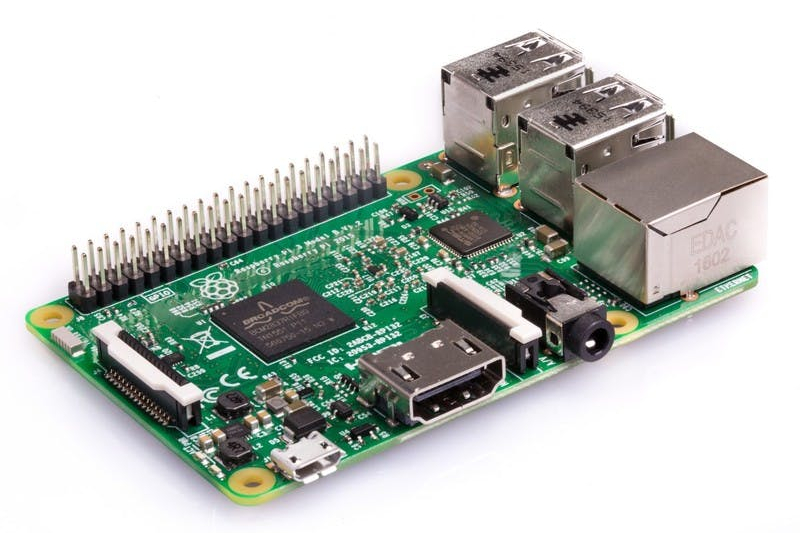
\includegraphics[width=\textwidth/2]{raspberry_pi_3b}
                \caption{Raspberry Pi 3B \cite{imagen_raspberry_pi_3b}\label{fig:ImagenRaspberryPi3B}}
            \end{figure}

            Se ha vuelto un producto tan popular que se vende para todo tipo de usos, desde centros
            multimedia \cite{centro_multimedia_raspberry_pi} o espejos inteligentes \cite{espejo_raspberry_pi}, hasta
            respiradores \cite{github_respirador} o este mismo proyecto.

        % subsection ¿Qué es Raspberry Pi? (end)

        \subsection{Modelos} % (fold)
        \label{sub:ModelosRaspberryPi}

            En sus ocho años de existencia, la Fundación Raspberry Pi ha lanzado cinco modelos de la Raspberry Pi, con
            diferentes variaciones. En la figura \ref{fig:ImagenModelosPi} se detallan alguno de los detalles de estos
            modelos \cite{raspberry_pi_wikipedia_en}:

            \begin{figure}[ht]
                \centering
                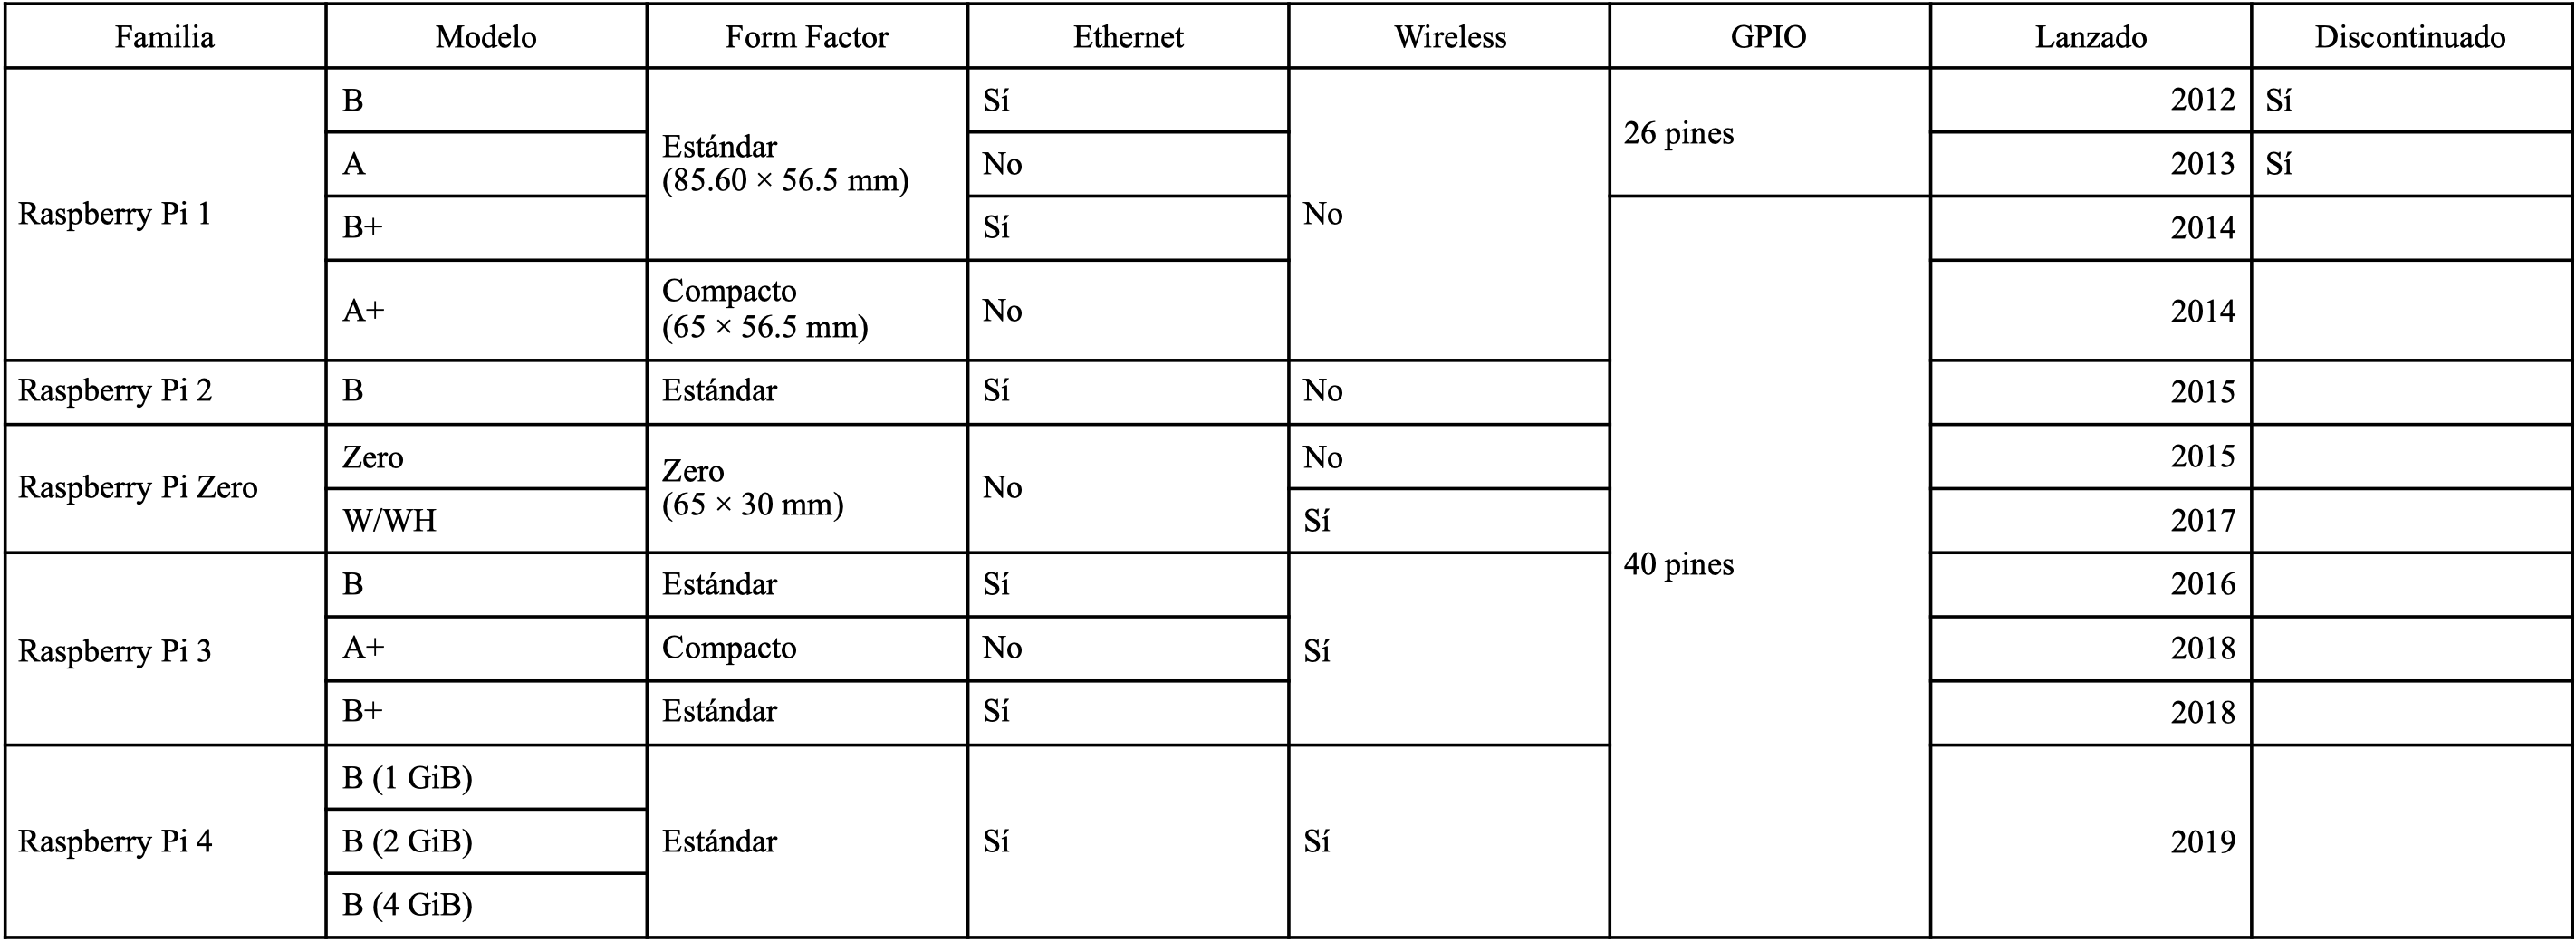
\includegraphics[width=\textwidth]{tabla_modelos_raspberry_pi}
                \caption{Tabla modelos de Raspberry Pi \cite{raspberry_pi_wikipedia_en}\label{fig:ImagenModelosPi}}
            \end{figure}

            \newpage

        % subsection Modelos (end)

        \subsection{Hardware} % (fold)
        \label{sub:HardwareRaspberryPi}

            La Raspberry Pi 3B utilizada en este proyecto tiene el siguiente hardware \cite{raspberry_pi_hardware}:

            \begin{itemize}
                \item \textbf{Procesador:} Broadcom BCM2837 de cuatro núcleos con arquitectura ARM Cortex A53 (ARMv8) a
                1.2 GHz.
                \item \textbf{Memoria:} 1GB de memoria LPDDR2
                \item \textbf{GPU:} Broadcom VideoCore IV a 250 MHz
                \item \textbf{USB:} Cuatro puertos USB 2.0.
                \item \textbf{GPIO:} Hay 40 pines de GPIO (General Purpose Input/Output). Estos pines funcionan a 3.3V.
                \item \textbf{Internet:} Ethernet 10/100 Mbit/s y WiFi 802.11 b/g/n
            \end{itemize}

        % subsection Hardware (end)

        \subsection{Alternativas} % (fold)
        \label{sub:AlternativasRaspberryPi}

            Podemos encontrar una gran variedad de alternativas, algunas de ellas son las
            siguientes \cite{alternativas_raspberry_pi}:

            \begin{itemize}
                \item \textbf{Orange Pi Prime}: Esta alternativa está viendo un gran crecimiento en los últimos años. La
                compañía que la fabrica se centra en precios más baratos y una gran personalización de la placa.
                \item \textbf{Banana Pi M3}: Puede compararse en prestaciones con la Raspberry Pi 3, sin embargo, el
                precio es mayor, ya que esta cuesta alrededor de \$80
                \item \textbf{ ASUS Tinker Board}: Es la más compatible a nivel de software, además, cuenta con más
                potencia de cálculo, lo que reduce los tiempos de procesamiento.
                \item \textbf{Huawei HiKey 960}: La alternativa de Huawei es la que cuenta con más potencia. Utiliza el
                procesador que utilizan los teléfonos de la compañía (Kirin 960). Pero también es la más cara, \$300.
            \end{itemize}

        % subsection Alternativas (end)

        \subsection{Lucha contra el Covid-19} % (fold)
        \label{sub:LuchaContraElCovid-19}

            Debido a la reciente crisis del coronavirus Covid-19, muchas personas empezaron a utilizar la Raspberry Pi
            para ayudar a luchar contra el virus. La principal utilidad que se encontró para esta placa en esa situación
            fue la de crear respiradores, pudiendo usar un código publicado en Github \cite{github_respirador} para
            programar la Raspberry Pi.

            Las ventas, por tanto, se dispararon, llegando a las 640.000 unidades vendidas en el mes de
            marzo \cite{ventas_raspberry_pi_covid}.

        % subsection Lucha contra el Covid-19 (end)

    % section Raspberry Pi (end)

    \section{Arduino} % (fold)
    \label{sec:Arduino}

        \subsection{¿Qué es Arduino?} % (fold)
        \label{sub:QueEsArduino}

            ``Arduino es una plataforma electrónica de código abierto basada en hardware y software fácil de usar. Las
            placas Arduino pueden leer entradas (luz en un sensor, un dedo en un botón o un mensaje de Twitter) y
            convertirlo en una salida: activar un motor, encender un LED, publicar algo online. Para hacerlo, utiliza
            el lenguaje de programación Arduino y el Software Arduino (IDE).''

            \begin{flushright}
                (Arduino, 2 de abril de 2020. \cite{arduino_introduction})
            \end{flushright}

            El proyecto Arduino nació en el año 2003 en el Interaction Design Institute Ivrea en Italia y, tanto la
            placa como el software que utiliza son open-source.

            \begin{figure}[ht]
                \centering
                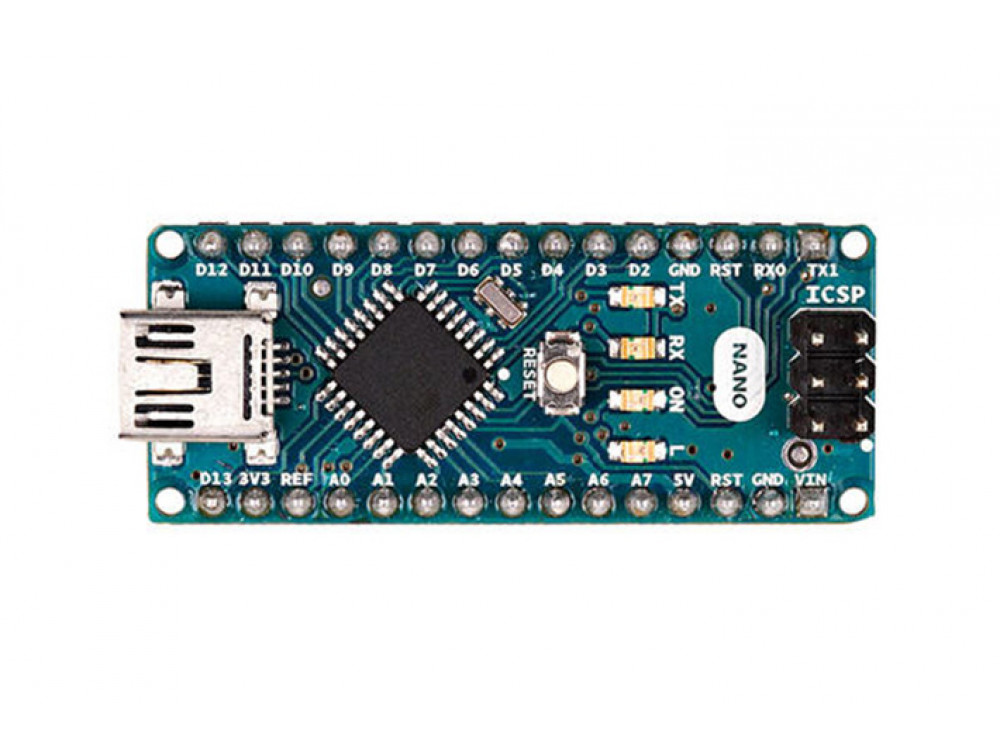
\includegraphics[width=\textwidth/2]{arduino_nano}
                \caption{Arduino Nano \cite{imagen_arduino_nano}\label{fig:ImagenArduinoNano}}
            \end{figure}

        % subsection ¿Qué es Arduino? (end)

        \subsection{Modelos} % (fold)
        \label{sub:ModelosArduino}

            En la figura \ref{fig:ImagenModelosArduino} se especifican los modelos de entrada de Arduino junto con algunas de sus
            especificaciones de hardware \cite{arduino_compare}:

            \begin{figure}[ht]
                \centering
                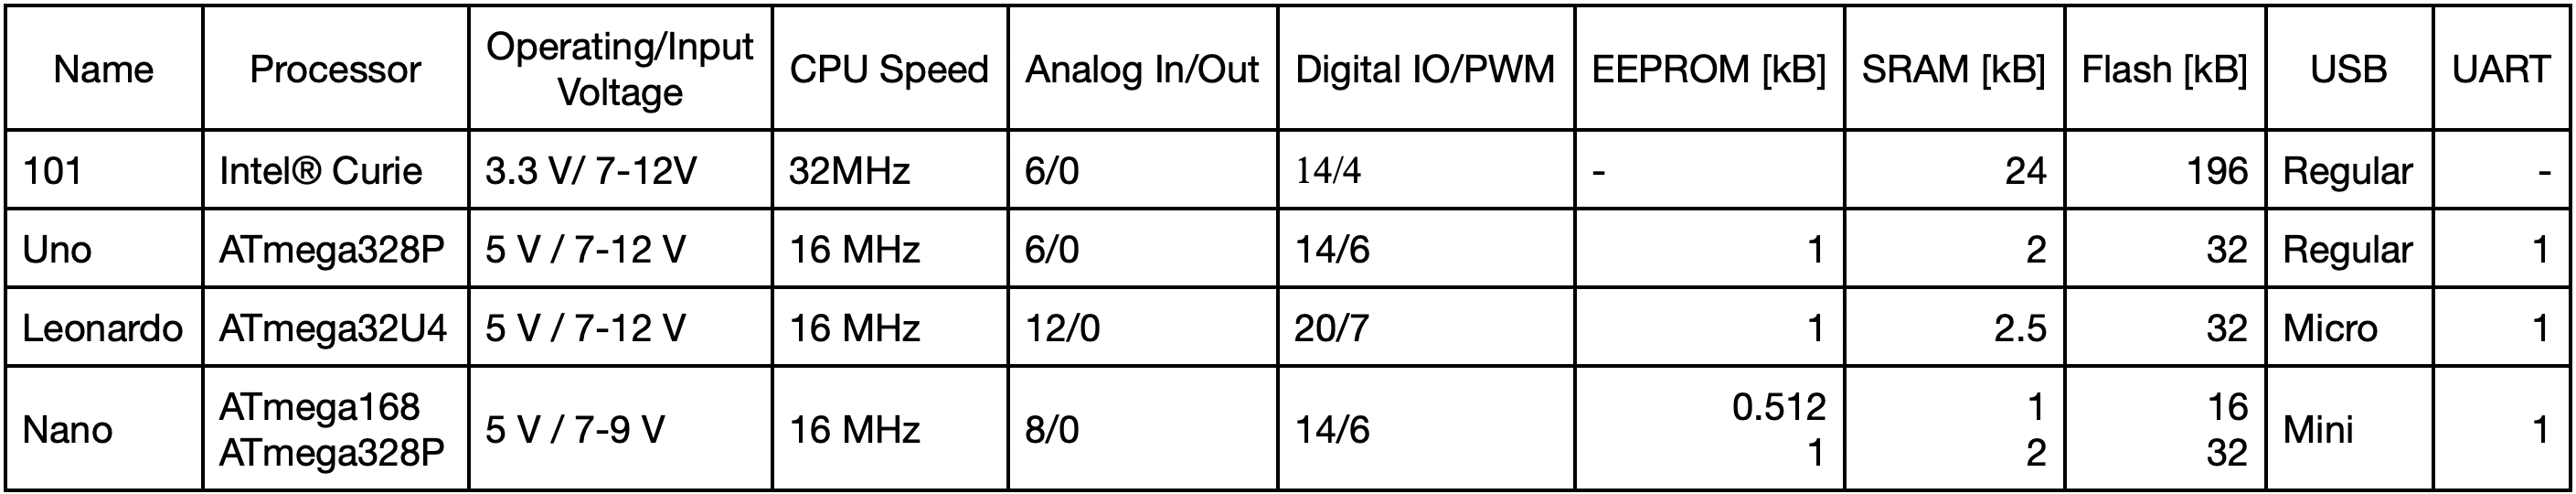
\includegraphics[width=\textwidth]{tabla_modelos_arduino}
                \caption{Tabla modelos de Arduino \cite{arduino_compare}\label{fig:ImagenModelosArduino}}
            \end{figure}

            El modelo utilizado en este proyecto es el Arduino Nano.

        % subsection Modelos (end)

        \subsection{Alternativas} % (fold)
        \label{sub:AlternativasArduino}

            Al igual que para Raspberry Pi (\ref{sub:AlternativasRaspberryPi}), hay una gran variedad de alternativas
            para la placa Arduino \cite{alternativas_arduino}:

            \begin{itemize}
                \item \textbf{NodeMCU}: Es la solución más barata. Además, añade la posibilidad de ejecutar código Lua.
                \item \textbf{Teensy 3}: Esta placa incluye un procesador más potente, haciéndola capaz de ejecutar
                tareas más pesadas. También se puede programar mediante el Arduino IDE, con la biblioteca Teensyduino.
                \item \textbf{MSP430 Launchpad}: Esta alternativa se centra en un consumo de energía más bajo que la
                Arduino.
            \end{itemize}

        % subsection Alternativas (end)

    % section Arduino (end)

    \section{Opciones actuales en el mercado} % (fold)
    \label{sec:OpcionesActualesEnElMercado}

        Son múltiples las baterías electrónicas a la venta. Una búsqueda rápida en Thomann \cite{thomann_baterias} nos
        muestra una gran variedad de baterías electrónicas en un amplío rango de precios, desde los 109\euro{} hasta los
        8.398\euro{}.

        \begin{figure}[ht]
            \centering
            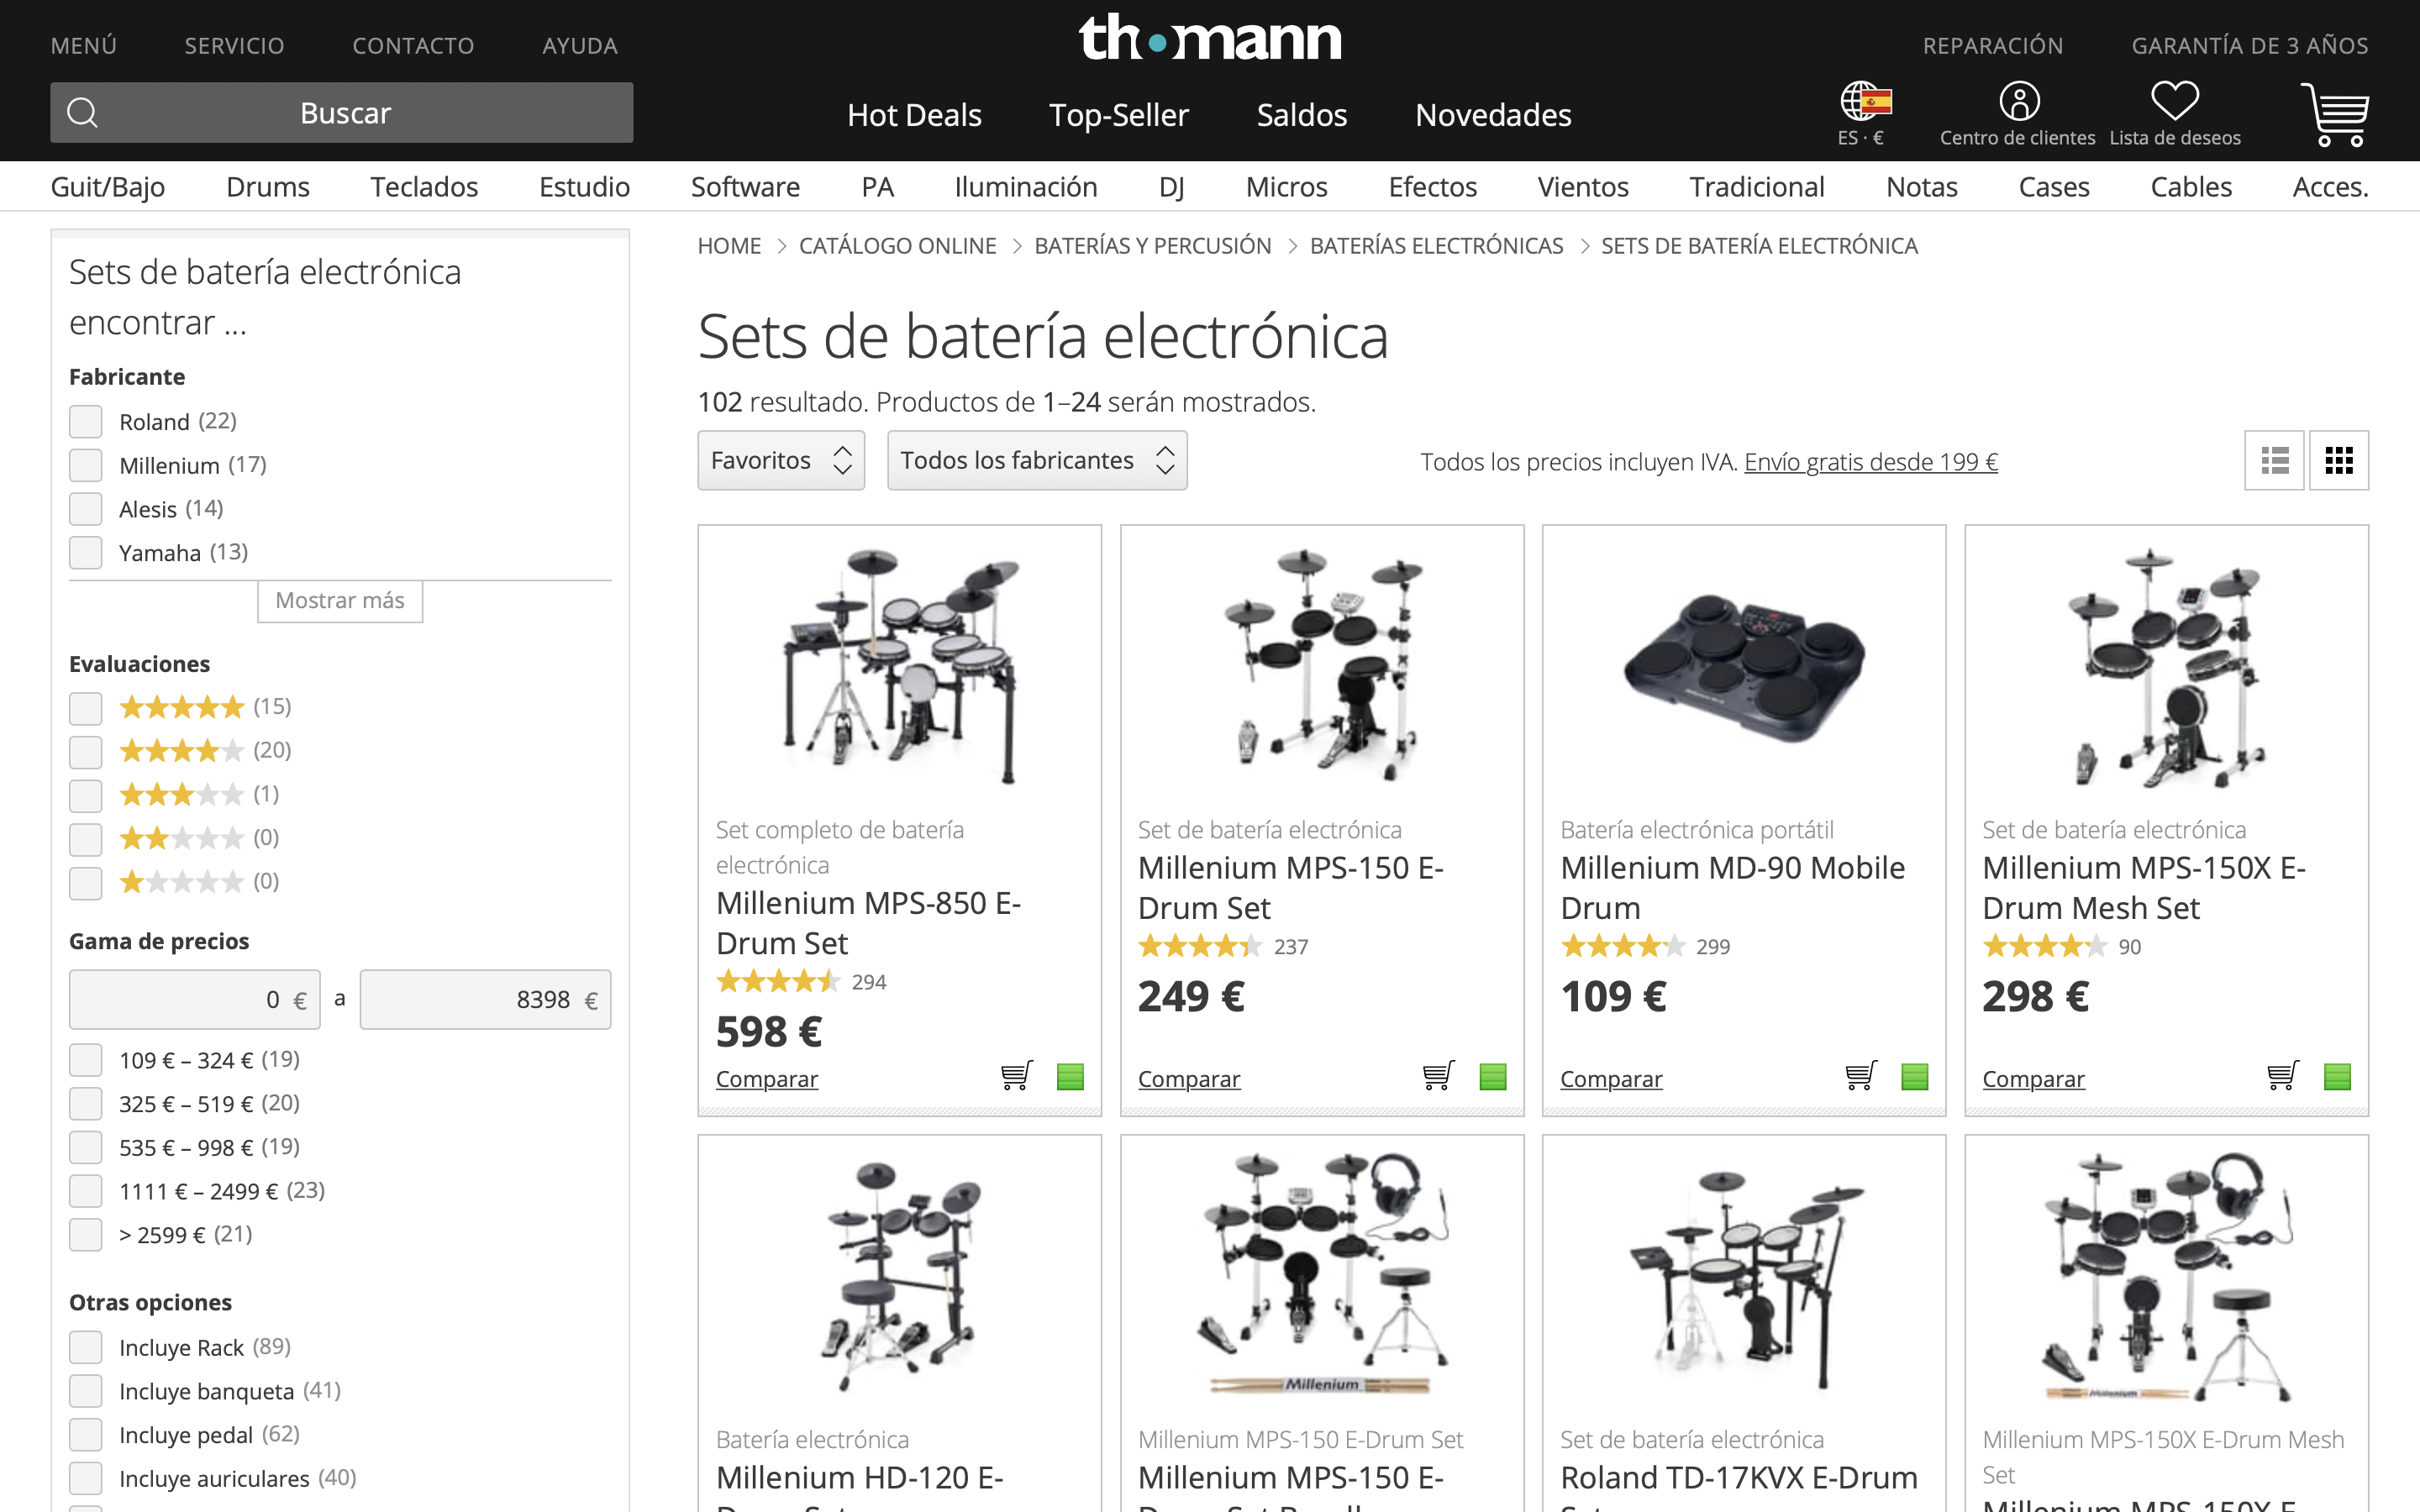
\includegraphics[width=\textwidth]{thomann_baterias}
            \caption{Resultados de la búsqueda de baterías electrónicas en Thomann \cite{thomann_baterias}
                     \label{fig:ThomannBusqueda}}
        \end{figure}

        \newpage

        En el terreno de las baterías que los usuarios se pueden construir (DIY), los principales resultados
        \cite{drum_magazine_diy_kit} utilizan elementos como sensores piezoeléctricos y sintetizadores MIDI. Los precios
        de estos sintetizadores van desde 150\euro{} a 2100\euro{}.

    % section Opciones actuales en el mercado (end)

    \section{Propuesta} % (fold)
    \label{sec:Propuesta}

        La propuesta que se presenta es un crear un programa de código abierto para que cualquier persona con unos
        conocimiento medios de informática pueda montar su propia batería electrónica en casa.

        Para completar con éxito el objetivo de este proyecto, los puntos más importantes serán:
        \begin{itemize}
            \item Reproducción del sonido con el menor delay posible.
            \item Reproducción de varios sonidos de manera concurrente.
            \item ...
        \end{itemize}

    % section Propuesta (end)

% chapter Estado del arte (end)

\newpage
